\usetikzlibrary{positioning}

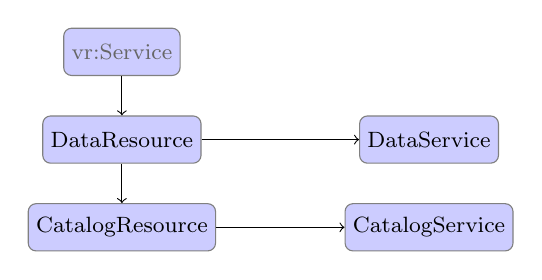
\begin{tikzpicture}[
class/.style={bottom color=blue!20,
  top color=blue!20,
  node distance=5mm and 20mm,
  rounded corners=1mm,
  minimum height=6mm,
  thin,draw=black!50,align=center,
  node font=\footnotesize
}]

\node (svc) [class,text=black!60] {vr:Service};
\node (dres) [class, below= of svc] {DataResource};
\node (dsvc) [class, right= of dres] {DataService};
\node (cres) [class, below= of dres] {CatalogResource};
\node (csvc) [class, below= of dsvc] {CatalogService};

\draw [black,->] (svc) to (dres);
\draw [black,->] (dres) to (dsvc);
\draw [black,->] (dres) to (cres);
\draw [black,->] (cres) to (csvc);

\end{tikzpicture}
